\section{Methodology}
\label{sec:methodology}
\begin{figure*}[t]
    \centering
    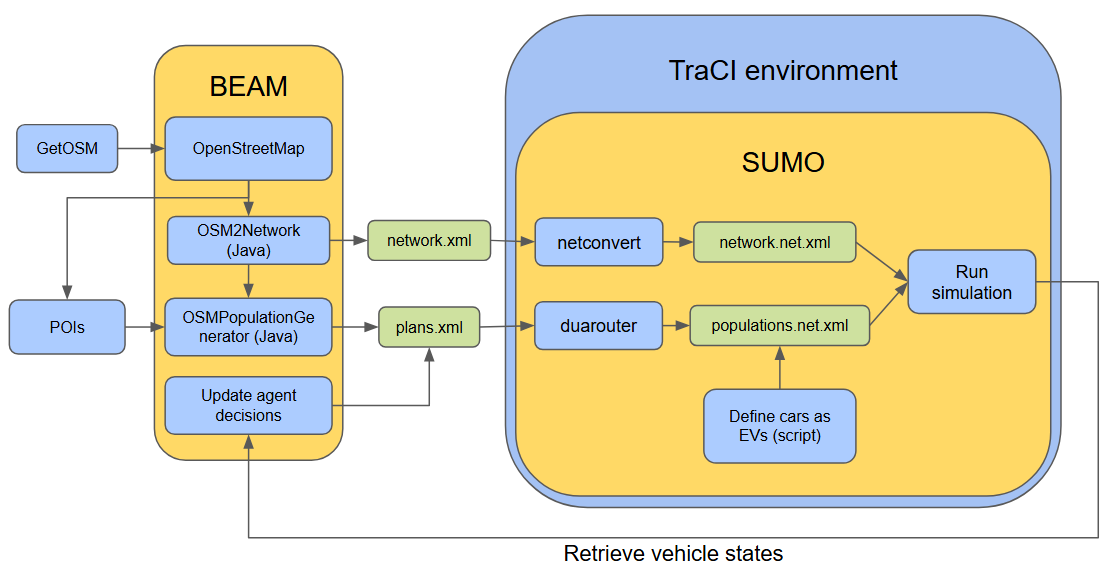
\includegraphics[width=0.8\textwidth]{images/Bild_BEAM_SUMO.png}
    \caption{Data Pipeline under BEAM and MATSim.}
    \label{fig:beam}
\end{figure*}

Initially our approach invovled MATSim for its high degree of configurability and its ability to simulate large-scale traffic networks, and when researching for a way increase the realism of our simulation, we incorporated BEAM (\cref{fig:beam}) -- which is an extension of MATSim. The pipeline begins with fetching data from OpenStreeMap, which is then processed and converted into a MATSim-compatible format. BEAM, which allows for real-time manipulation, is then used to simulate traffic flows and charging behavior.
However, we found its lack of deterministic execution, high error rates, and the need for extensive calibration to be a barrier to producitivty and reproducibility. We therefore switched to SUMO and TraCI completely, which provides a more stable and deterministic simulation environment, while still allowing for detailed and dynamic modeling of traffic flows and charging behavior. 

As of now, we are using SUMO as a microscopic traffic simulator and TraCI with a grid impact model and a statistical distribution for home-charging devices to evaluate the spatial distribution of bidirectional charging stations. Two algorithms are implemented to test different siting strategies: 

\begin{itemize}
    \item \textbf{Saturate-and-Prune}: A naive iterative approach where candidate locations cover all road segments, ensuring maximum accessibility. After each trial execution, charging stations with less than a 5\% utilization rate are removed, and the simulation is rerun until all remaining stations exceed this threshold.
    \item \textbf{Clustering}: A heuristic that prioritizes locations with high traffic flow, potential traffic congestions and consideration for low state of charge. The flow of traffic determines the placement of charging stations, with the goal of maximizing accessibility in spots where vehicles are most likely to need charging and decreasing the likelihoof of detours.
\end{itemize}

\subsection{System Overview}

\begin{figure*}[t]
    \centering
    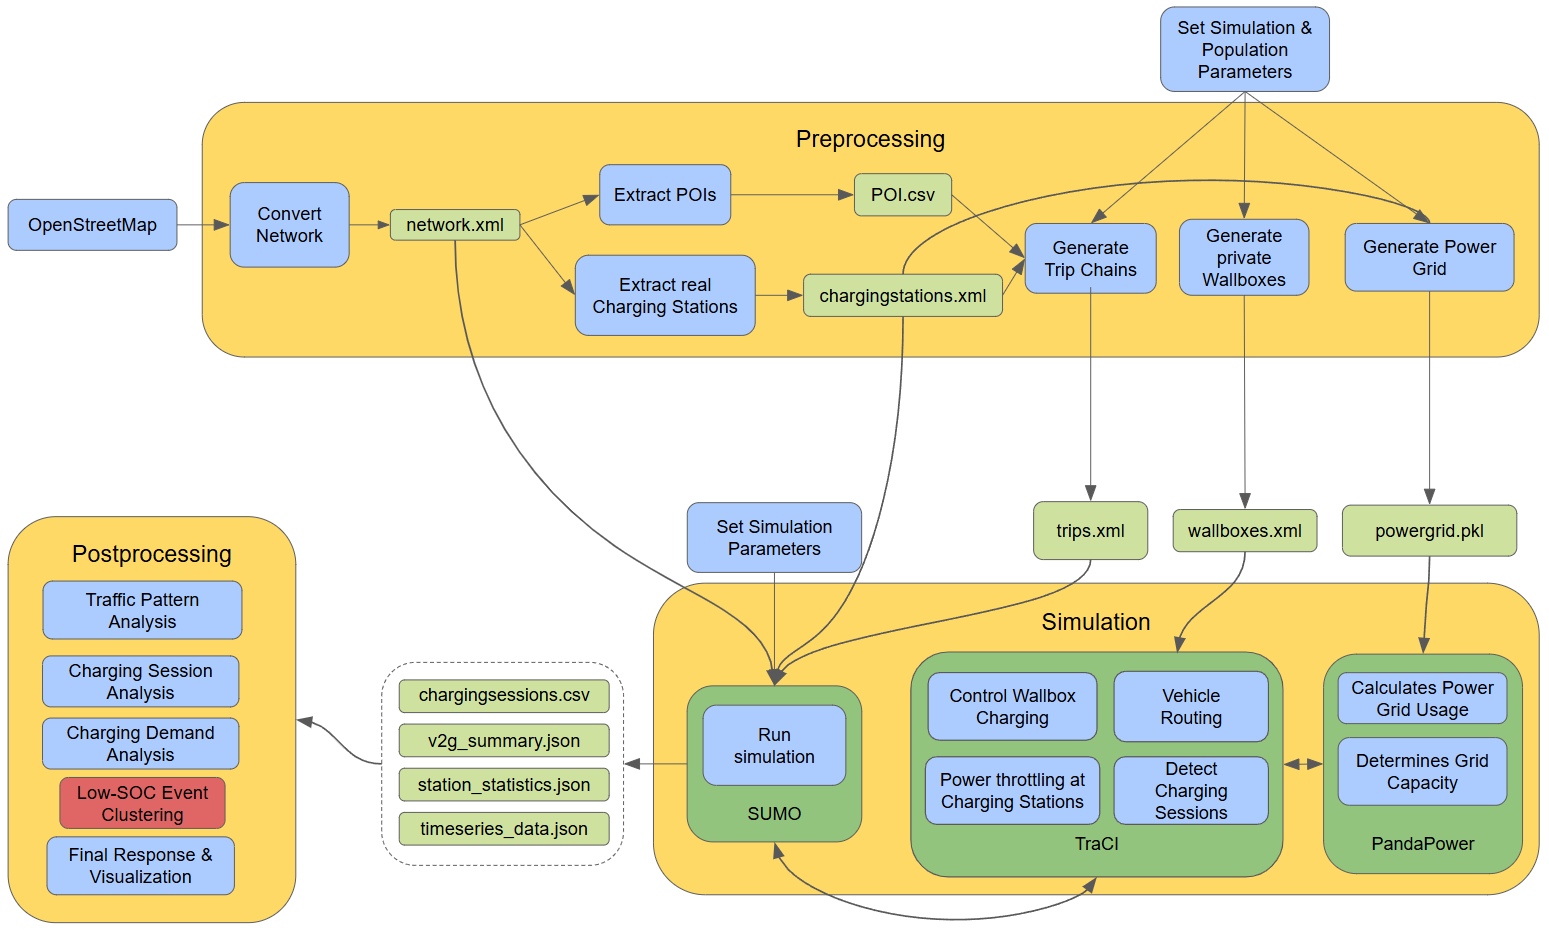
\includegraphics[width=0.9\textwidth]{images/data_pipeline.png}
    \caption{Complete Data Pipeline}
    \label{fig:data_pipeline}
\end{figure*}

